\documentclass[11pt,a4paper]{article}

\usepackage[margin=1in]{geometry}
\usepackage{amsmath,amssymb,amsthm}
\usepackage{booktabs}
\usepackage{array}
\usepackage{listings}
\usepackage{xcolor}
\usepackage[expansion=false]{microtype}
\usepackage{enumitem}
\usepackage{tikz}
\usepackage{float}
\usepackage[hidelinks]{hyperref}

\usetikzlibrary{arrows,decorations.pathmorphing,calc}
\tikzset{>=stealth'}

\definecolor{codebg}{HTML}{F5F5F5}
\definecolor{ribL}{HTML}{7F77DD}
\definecolor{ribR}{HTML}{1D9E75}
\definecolor{amb}{HTML}{EF9F27}

\lstset{
  basicstyle=\ttfamily\footnotesize,
  backgroundcolor=\color{codebg},
  frame=single, framesep=4pt, rulecolor=\color{black!20},
  breaklines=true, columns=fullflexible, keepspaces=true,
  showstringspaces=false, xleftmargin=0pt, aboveskip=1em, belowskip=1em
}

\newcommand{\MUST}{\textsc{must}}
\newcommand{\MUSTNOT}{\textsc{must not}}
\newcommand{\SHOULD}{\textsc{should}}
\newcommand{\SHOULDNOT}{\textsc{should not}}
\newcommand{\MAY}{\textsc{may}}

\theoremstyle{definition}
\newtheorem{definition}{Definition}
\theoremstyle{plain}
\newtheorem{proposition}{Proposition}
\theoremstyle{remark}
\newtheorem*{decision}{Decision required}

% ---------------------------------------------------------------- scene macros
\newcommand{\spools}{%
  \fill[ribL,opacity=.45,rounded corners=2pt] (1.55,5.40) rectangle (2.45,5.95);
  \fill[ribR,opacity=.45,rounded corners=2pt] (5.55,5.40) rectangle (6.45,5.95);
  \node[font=\scriptsize] at (2,6.22) {left spool};
  \node[font=\scriptsize] at (6,6.22) {right spool};
}
\newcommand{\musician}{%
  \draw[gray] (4,-0.10) circle (0.23);
  \node[font=\scriptsize] at (4,-0.10) {M};
}
\newcommand{\axes}{%
  \draw[->,gray,thin] (0.85,4.30) -- (1.45,4.30) node[right,font=\scriptsize]{$x$};
  \draw[->,gray,thin] (0.85,4.30) -- (0.85,4.90) node[above,font=\scriptsize]{$z$};
}
\newcommand{\ribbonsopen}{%
  \draw[ribL,opacity=.45,line width=16pt,line join=round]
    (2,5.40) -- (2,4.60) -- (3.10,4.00) -- (3.10,0.70);
  \draw[ribR,opacity=.45,line width=16pt,line join=round]
    (6,5.40) -- (6,4.60) -- (4.90,4.00) -- (4.90,0.70);
}
\newcommand{\ribbonszipped}{%
  \draw[ribL,opacity=.45,line width=16pt,line join=round]
    (2,5.40) -- (2,4.60) -- (3.72,4.20) -- (3.72,2.20) -- (3.10,1.70) -- (3.10,0.70);
  \draw[ribR,opacity=.45,line width=16pt,line join=round]
    (6,5.40) -- (6,4.60) -- (4.28,4.20) -- (4.28,2.20) -- (4.90,1.70) -- (4.90,0.70);
}
\newcommand{\mesh}[2]{%
  \draw[gray!75,decorate,decoration={zigzag,segment length=5pt,amplitude=3pt}]
    (4,#1) -- (4,#2);
}
\newcommand{\mountclips}{%
  \fill[amb,opacity=.75,rounded corners=1pt] (3.76,1.05) rectangle (3.92,1.45);
  \fill[amb,opacity=.75,rounded corners=1pt] (4.08,1.05) rectangle (4.24,1.45);
}
\newcommand{\handat}[2]{\filldraw[fill=white,draw=gray!80,thin] (#1,#2) circle (0.17);}
\newcommand{\headroll}[2]{%
  \begin{scope}[shift={(#1,#2)},scale=0.62]
    \draw[gray] (0,0) circle (0.42);
    \draw[gray!70,thin,dashed] (0,-0.55) -- (0,0.62);
    \draw[gray,thick,rotate=20] (0,-0.50) -- (0,0.58);
    \draw[->,amb,thick] (-0.10,0.80) to[out=20,in=150] (0.42,0.62);
  \end{scope}}
\newcommand{\handsdefault}{\handat{3.10}{0.55}\handat{4.90}{0.55}}

\title{\textbf{The F1R3Skein Virtual Instrument}\\[0.3em]
\large Specification, revision 4}
\author{F1R3FLY.io}
\date{4 September 2026}

\begin{document}
\maketitle

\begin{abstract}
\noindent
This document specifies the F1R3Skein virtual instrument: the gestural surface through which a
musician draws melody out of the digit streams of mathematical constants, and out of which the
platform's two primary artifacts---tunes and performances---are produced.

Revision 3 replaced the instrument's physical model. Revision 4 settles the ten decisions that
model raised and adds the organising principle that had been missing:

\begin{quote}
\textbf{While M holds the ribbons she is playing. While the ribbons are mounted she is in meta
play.}
\end{quote}

That principle removes machinery rather than adding it. What revision 3 specified as a
suppression rule---``pull must be inhibited during a cut''---is not a rule at all: pull does not
exist in meta play because there are no ribbons in her hands to pull. The recogniser evaluates one
mode's predicates at a time.

Also settled here: the cut is \emph{virtual}, so the band is never severed; the zip wave has a
bounded frontier and the far field compresses so that long plays visibly cost depth; tempo is read
from the speed at which M closes her hands and is fixed for the life of a mesh; and halt is a head
gesture, which removes the eyes from the vocabulary entirely and with them the visionOS gaze
constraint that dominated revision 3.

The vocabulary is ten gestures, each with a diagram. Section~\ref{sec:decisions} lists what
remains open, and \S\ref{sec:demo} triages the set against a demo deadline.
\end{abstract}

\tableofcontents

\section{Scope and conformance}

In scope: the generative core, the playing surface and its geometry, the instrument's state model,
the gesture vocabulary and its detection criteria, the wire protocol, the visual and audio models,
performance recording, and the budgets that make the instrument playable.

Out of scope: identity, galleries, the engagement ledger, breeding and selection, and the on-chain
representation of tunes. This document defines what the instrument \emph{produces}. The instrument
is to be brought up and proven standalone; wiring it to a shard follows, and nothing here \MAY{}
be made to depend on shard availability.

\MUST, \MUSTNOT, \SHOULD, \SHOULDNOT{} and \MAY{} are used in the sense of RFC 2119.
\emph{M} denotes the musician throughout.

\subsection{Terminology}

\begin{description}[leftmargin=2.4cm,style=nextline,font=\normalfont\itshape]
\item[Engine] The process holding authoritative instrument state.
\item[Client] The visionOS application: gesture recognition, rendering, audio.
\item[Stream] One spigot: a constant, an output base, a cursor position.
\item[Spool] The visible source of one stream, far from M on the $z$-axis.
\item[Ribbon] The visible material spooling from one spool toward M.
\item[Notch] One digit position, presented on a ribbon's inner edge.
\item[Skein] The pair of ribbons together with their relative registration.
\item[Zip front] The boundary where unmeshed ribbon becomes meshed. The playhead.
\item[Tune] A snipped, named artifact.
\item[Performance] The recorded trace of a session.
\end{description}

\section{Deployment configurations}

\begin{description}[leftmargin=1cm,style=nextline]
\item[\textbf{S1 --- Tethered.}] Engine on a Mac, client on the headset, TCP over the local network
with Bonjour discovery. September test configuration; explicitly a stopgap.
\item[\textbf{S2 --- On-device.}] Engine built for \texttt{arm64-apple-visionos} as a
static library behind a C foreign-function interface. No transport at all. The target.
\end{description}

The protocol of Section~\ref{sec:protocol} is defined over an abstract bidirectional channel; in S1
that is a TCP stream, in S2 a pair of FFI ring buffers. No other part of this specification
distinguishes them, and the client \MUSTNOT{} contain transport-specific logic outside its channel
implementation.

The Unix-domain-socket transport \MUSTNOT{} be used for device testing: a Unix socket is addressed
by a path in one host's filesystem, and the headset is a different host.

\section{The generative core}

\subsection{Streams}

The engine \MUST{} provide the five constants---$\pi$, $e$, $\varphi$, $\ln 2$, Liouville's---each
emitting digits in a configurable base $b$, $2 \le b \le 36$. Emission \MUST{} be exact and
unbounded. A stream configuration is a pair $(c,b)$; with a cursor position $p$ it determines the
digit $d(c,b,p)$ uniquely.

The $\pi$ implementation \SHOULD{} move to Bailey--Borwein--Plouffe extraction where the base
permits, and \MUST{} memoise emitted digits so re-realisation of a visited range is $O(1)$ per
digit. Deep positions are exactly what a long session produces.

\subsection{Two cursors, separately mobile}

The skein holds two configurations and two \emph{independent} cursor positions, $p_L$ and $p_R$.
Independence is the point of the design and \MUST{} be preserved: it is what lets M hold a rhythmic
motif fixed while advancing pitch, or dually.

\begin{proposition}[The instrument performs its own algebra]
Holding one ribbon fixed and meshing a different segment of the other against it takes the
durations of one candidate and the pitches of another. That is the crossover operator
$\mathsf{XPitch}$ of the breeding engine, performed by hand; its dual is
$\mathsf{XPitch}(f,m)$ by the rectangular-band identity. Selection and reproduction are not a
subsystem bolted onto a music toy---the population does at scale what M does at the bench.
\end{proposition}

\subsection{Note mapping}

\label{sec:maps}
One stream governs pitch, the other duration; \emph{twist} exchanges the roles. For the $k$-th
meshed notch pair the engine \MUST{} produce
$(\Pi(d_{\text{pitch}}),\ \Delta(d_{\text{duration}}))$. Both maps \MUST{} be session parameters,
not build constants. Pitch maps \MUST{} include major, minor, pentatonic major, pentatonic minor,
Dorian, whole tone and chromatic over a configurable root; duration maps \MUST{} include musical,
linear, exponential and fixed. A stream's base \SHOULD{} match the cardinality of the map it drives.

Both maps \MUST{} be changeable during a session. For the first release the control is
\textbf{textual}, in the panel, and \MUSTNOT{} consume a gesture: the vocabulary is already at
ten, and choosing a scale is a settings act rather than a performing one. A gestural treatment may
follow. Because a changed map changes how an existing term sounds, the capture envelope of
\S\ref{sec:envelope} carries the maps in force at the moment of capture.

\section{The playing surface}
\label{sec:surface}

Axes are M's: $x$ is left--right, $y$ is up--down, $z$ is depth away from M.

Each stream has its own spool. The two spools sit at the \emph{same height} and are spread apart on
the $x$-axis, far from M on $z$. Ribbon spools from each toward M's hands. Each ribbon divides into
three sections:

\begin{description}[leftmargin=1.6cm,style=nextline]
\item[\textbf{Future}] still wound on the spool, unseen.
\item[\textbf{Present}] between the spool and M's hands, visible.
\item[\textbf{Past}] having passed the hands, hanging below them toward the floor.
\end{description}

Each ribbon carries notches on its \emph{inner} edge---the edge facing the other ribbon. Bringing
the ribbons together meshes the notches over a section of the present, leaving unmeshed margins
near the hands and near the spools. The mount sits between the ribbons, just in front of the hands,
and is a pair of clips.

\begin{figure}[H]\centering
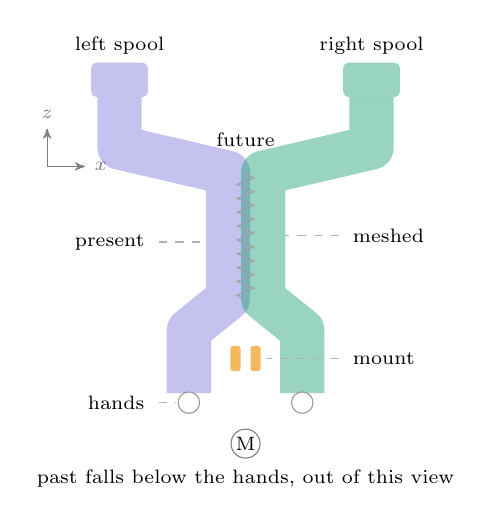
\begin{tikzpicture}[scale=0.80]
\axes \spools \ribbonszipped \mesh{2.20}{4.20} \mountclips \handsdefault \musician
\node[font=\scriptsize] at (4,4.72) {future};
\node[font=\scriptsize,anchor=east] at (2.55,3.10) {present};
\draw[gray!60,thin,dashed] (2.62,3.10) -- (3.38,3.10);
\node[font=\scriptsize,anchor=west] at (5.55,3.20) {meshed};
\draw[gray!60,thin,dashed] (5.48,3.20) -- (4.62,3.20);
\node[font=\scriptsize,anchor=west] at (5.55,1.25) {mount};
\draw[gray!60,thin,dashed] (5.48,1.25) -- (4.32,1.25);
\node[font=\scriptsize,anchor=east] at (2.55,0.55) {hands};
\draw[gray!60,thin,dashed] (2.62,0.55) -- (2.90,0.55);
\node[font=\scriptsize] at (4,-0.65) {past falls below the hands, out of this view};
\end{tikzpicture}
\caption{The playing surface, seen from above. Two spools at the same height, spread on $x$.}
\end{figure}

\begin{quote}
\textbf{A notch pair is a note.} Meshing commits notch $k$ on the left to notch $k$ on the right.
While unmeshed the ribbons slide independently and M sets the relative phase; once meshed the
pairing is fixed. Independent mobility and well-formed pairing are not in tension---they are
separated in time by the zip.
\end{quote}

\section{Instrument state}

\[
\Sigma = \big\langle\;
(c_L,b_L,p_L),\; (c_R,b_R,p_R),\;
m,\; \zeta,\; \lambda,\;
\Pi,\Delta,\tau,\iota,\; T
\;\big\rangle
\]

with $m \in \{\textsf{play}, \textsf{meta}\}$ the mode, $\zeta$ the zip state (unzipped, or
zipped with a front position, a propagation state and a frontier budget), $\lambda$ the loop
state, $\tau$ the tempo of the current mesh, $\iota$ the instrument, $T$ the tray. The client
\MUSTNOT{} hold authoritative state; it renders $\Sigma$ and emits gestures.

\subsection{The two modes}

\begin{center}
\begin{tabular}{lll}
\toprule
 & \textbf{Play} & \textbf{Meta} \\
\midrule
Ribbons        & in M's hands            & in the mount clips \\
Wave           & propagating, or halted  & stopped \\
Gestures       & pull, twist, zip, unzip, halt & loop, scissors \\
Transition out & mount                   & unmount \\
\bottomrule
\end{tabular}
\end{center}

The recogniser \MUST{} evaluate only the active mode's predicates. This is not an optimisation: it
is what makes the vocabulary safe. Travelling a hand along $z$ to bracket a cut is
indistinguishable from a pull, and the two never collide only because pull does not exist in meta
play.

Mounting while unzipped is permitted and yields a meta play in which loop and scissors are both
unavailable, there being nothing meshed to loop or to cut.

\section{Gesture vocabulary}
\label{sec:gestures}

Ten gestures, grouped by mode. Each is given with its physical form, its effect, and a diagram of
the surface during it.

\subsection{Pull \normalfont(play)}

M draws one hand toward herself, advancing that stream. Step count is proportional to speed. Pulls
are per-hand and independent; this is where the relative phase between the two streams is set.

\begin{figure}[H]\centering
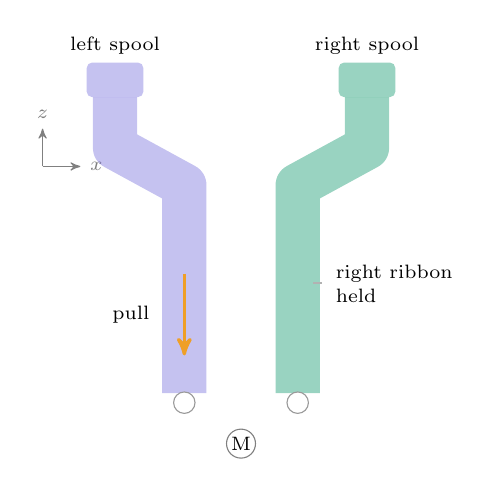
\begin{tikzpicture}[scale=0.80]
\axes \spools \ribbonsopen \handsdefault \musician
\draw[->,amb,very thick] (3.10,2.60) -- (3.10,1.30);
\node[font=\scriptsize,anchor=east] at (2.70,1.95) {pull};
\node[font=\scriptsize,anchor=west] at (5.35,2.60) {right ribbon};
\node[font=\scriptsize,anchor=west] at (5.35,2.25) {held};
\draw[gray!60,thin,dashed] (5.28,2.45) -- (5.12,2.45);
\end{tikzpicture}
\caption{Pull. Ribbons unmeshed; each advances alone. Holding one and pulling the other is how M
chooses which rhythm meets which pitches.}
\end{figure}

\subsection{Twist \normalfont(play)}

One hand held clearly above the other, hands apart. Exchanges the two streams, cursors included.
Twist \MUST{} be permitted only while unzipped: the mesh commits the pairing, and exchanging roles
underneath a committed mesh has no coherent reading.

\begin{figure}[H]\centering
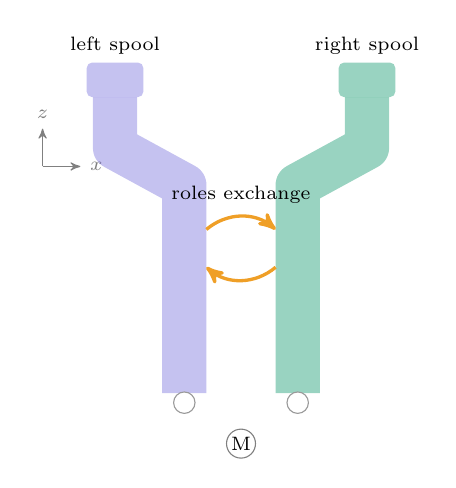
\begin{tikzpicture}[scale=0.80]
\axes \spools \ribbonsopen \handsdefault \musician
\draw[->,amb,very thick] (3.45,3.30) to[out=40,in=140] (4.55,3.30);
\draw[->,amb,very thick] (4.55,2.70) to[out=220,in=320] (3.45,2.70);
\node[font=\scriptsize] at (4,3.85) {roles exchange};
\end{tikzpicture}
\caption{Twist. Which stream governs pitch and which governs duration is swapped. Permitted only
while unzipped.}
\end{figure}

\subsection{Zip \normalfont(play)}
\label{sec:zip}

M brings the two ribbons together. The notches mesh, and \textbf{the mesh keeps going}: the zip
front propagates away from M into the future without further input. The zip front is the playhead
--- each notch pair sounds as it engages.

\paragraph{Tempo is read from the closing.} The speed at which M's hands come together sets the
propagation rate. The client \MUST{} measure closing speed over a short window \emph{before} the
zip threshold is crossed, not at the crossing frame, or the tempo will be noisy.

\paragraph{One tempo per mesh.} Halting and resuming involves no closing motion, so there is no new
speed to read and the tempo carries over. A mesh therefore has a single tempo for its whole life,
from the zip that created it until it is unzipped. This is a simplification worth keeping: it makes
a captured region's tempo unambiguous.

\paragraph{The frontier is bounded.} The wave \MUST{} stop of its own accord after
\texttt{zip.frontier\_max} notches. The bound is the length of a generous looper phrase --- on the
order of $10^{3}$ notches at a few notes per second --- and \SHOULD{} be set from a reference
device rather than guessed. Long before the bound is reached the spools \MUST{} have compressed
toward point sources, so that a long play visibly costs $z$-axis real estate.

There is an alignment here that is not contrived: a long play costs depth in the scene and costs
phlo in the engine, because deep cursor positions are more expensive to realise. The metaphor and
the economics say the same thing.

\begin{figure}[H]\centering
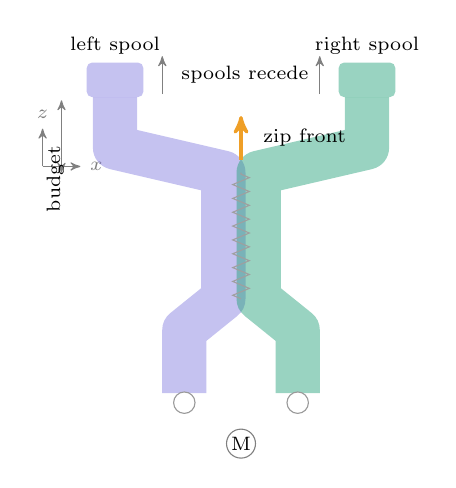
\begin{tikzpicture}[scale=0.80]
\axes \spools \ribbonszipped \mesh{2.20}{4.20} \handsdefault \musician
\draw[->,amb,very thick] (4,4.40) -- (4,5.10);
\node[font=\scriptsize,anchor=west] at (4.20,4.75) {zip front};
\draw[->,gray,thin] (2.75,5.45) -- (2.75,6.05);
\draw[->,gray,thin] (5.25,5.45) -- (5.25,6.05);
\node[font=\scriptsize,anchor=west] at (2.90,5.75) {spools recede};
\draw[<->,gray,thin] (1.15,4.20) -- (1.15,5.35);
\node[font=\scriptsize,anchor=east,rotate=90] at (1.05,4.78) {budget};
\end{tikzpicture}
\caption{Zip. The wave propagates unaided; the spools retreat to feed it, up to a bounded frontier.
The closing speed of the hands set the tempo.}
\end{figure}

\subsection{Halt \normalfont(play)}
\label{sec:halt}

M tilts her head to stop the wave. The front freezes, the mesh is untouched, and the ribbons stay
in her hands. \textbf{She has not stopped performing --- she has stopped the generation of music.}
Halt is how M places a silence longer than any rest the duration stream will hand her, and it is
the only gesture in the vocabulary that composes rather than manages.

\paragraph{Why the head.} Halt is the one transport control M needs while both hands are committed
to holding ribbons. Head pose is available to applications --- it is the channel analytics vendors
fall back on precisely because gaze is not --- and it is otherwise idle during play. The vocabulary
then divides cleanly: hands move material, head handles transport. The authorization requirements
of the device-pose provider \MUST{} be confirmed before this is built.

\paragraph{Roll, not pitch or yaw.} Yaw is in constant use, as M looks between the tray, the spools
and the front. Pitch is what people do to keep time, and nodding along would fire it continuously.
Roll is the least-used axis in ordinary playing --- though not unused, since players lean into a
phrase by reflex, so the threshold \MUST{} be generous, \MUST{} require a hold, and \MUST{} live in
the calibration profile.

\paragraph{Set and clear, not toggle.} One direction halts, the other resumes; a repeat in the same
direction is a no-op. A toggle on a noisy detector is unsafe: a missed fire and a double fire are
indistinguishable to M, and she will correct by tilting again, which under a toggle undoes the
correction. The gesture \MUST{} be edge-triggered with hysteresis, firing near $15^\circ$ and
re-arming below $6^\circ$, requiring a return to near-upright between firings. This matches the
direction-sensitive treatment of loop, so the two feel consistent.

\paragraph{Confirmation and equivalence.} A head tilt is proprioceptively silent --- it does not
feel like an action the way closing the hands does --- so the freezing of the front \MUST{} be
given unmistakable visual confirmation. A panel equivalent \MUST{} exist, since a head-only control
is unavailable to anyone who cannot tilt comfortably.

\begin{figure}[H]\centering
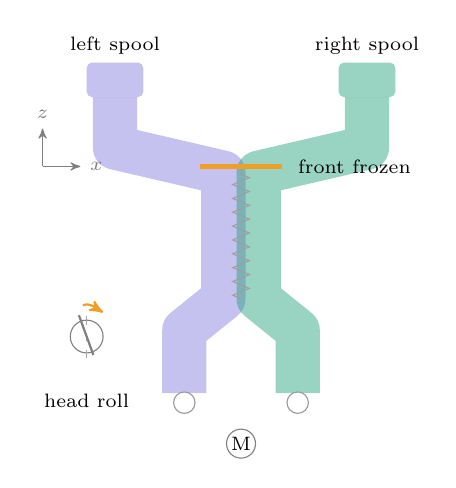
\begin{tikzpicture}[scale=0.80]
\axes \spools \ribbonszipped \mesh{2.20}{4.20} \handsdefault \musician
\draw[amb,line width=2pt] (3.35,4.30) -- (4.65,4.30);
\node[font=\scriptsize,anchor=west] at (4.75,4.30) {front frozen};
\headroll{1.55}{1.60}
\node[font=\scriptsize,anchor=north] at (1.55,0.85) {head roll};
\end{tikzpicture}
\caption{Halt. A head tilt freezes the front; the mesh and the tempo survive. The opposite tilt
resumes, and the tempo carries over because there is no closing motion to read a new one from.}
\end{figure}

\subsection{Unzip \normalfont(play)}

Separates the ribbons, retiring the mesh from the near end. Unzipping is what lets M re-set the
relative phase and mesh a different segment against a held ribbon --- the crossover move of
Proposition~1. It is also the only way to change tempo, since a new mesh takes a new closing speed.

\begin{figure}[H]\centering
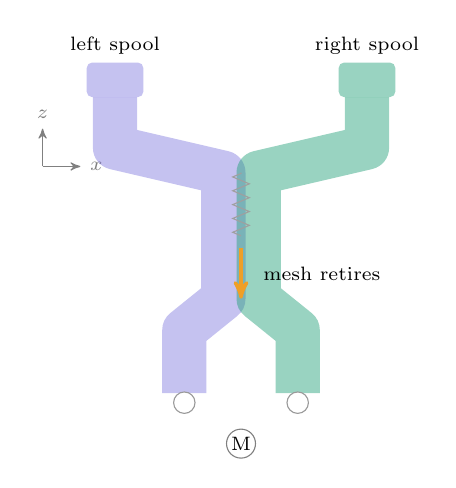
\begin{tikzpicture}[scale=0.80]
\axes \spools \ribbonszipped \mesh{3.20}{4.20} \handsdefault \musician
\draw[->,amb,very thick] (4,3.00) -- (4,2.20);
\node[font=\scriptsize,anchor=west] at (4.20,2.60) {mesh retires};
\end{tikzpicture}
\caption{Unzip. The pairing is released from the near end, freeing the ribbons to slide
independently again.}
\end{figure}

\subsection{Mount \normalfont(play $\to$ meta)}

M slots the unmeshed lead of each ribbon into the clips. Mounting \textbf{stops the wave} and
enters meta play. It is a clear gestural declaration that M is about to do something else with her
hands, and the mount takes over the holding so that both hands are free to travel out along the
meshed band. The mount contributes no boundary to any captured tune.

\begin{figure}[H]\centering
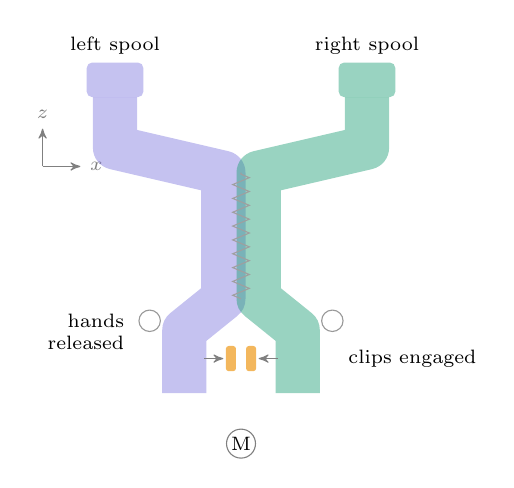
\begin{tikzpicture}[scale=0.80]
\axes \spools \ribbonszipped \mesh{2.20}{4.20} \mountclips \musician
\handat{2.55}{1.85}\handat{5.45}{1.85}
\draw[->,gray,thin] (3.42,1.25) -- (3.72,1.25);
\draw[->,gray,thin] (4.58,1.25) -- (4.28,1.25);
\node[font=\scriptsize,anchor=west] at (5.55,1.25) {clips engaged};
\node[font=\scriptsize,anchor=east] at (2.30,1.85) {hands};
\node[font=\scriptsize,anchor=east] at (2.30,1.50) {released};
\end{tikzpicture}
\caption{Mount. Two clips take the load, the wave stops, and M enters meta play.}
\end{figure}

\subsection{Unmount \normalfont(meta $\to$ play)}

M reaches into the clips and takes the ribbons back. \textbf{The mesh survives.} She picks up a
still-zipped assembly with the wave stopped, and resumes propagation from the current front --- at
the mesh's existing tempo, by \S\ref{sec:zip}. The session rhythm is play, capture, play.

\begin{figure}[H]\centering
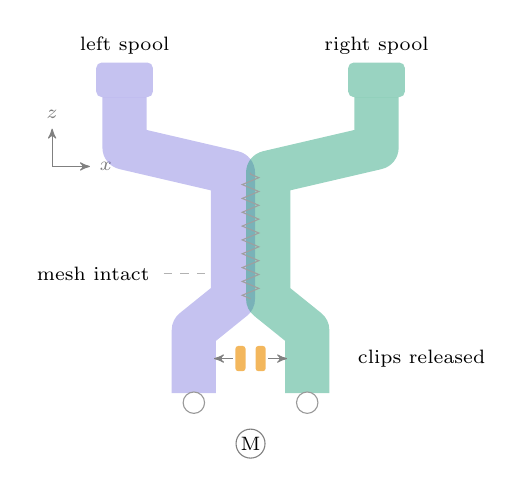
\begin{tikzpicture}[scale=0.80]
\axes \spools \ribbonszipped \mesh{2.20}{4.20} \mountclips \handsdefault \musician
\draw[->,gray,thin] (3.72,1.25) -- (3.42,1.25);
\draw[->,gray,thin] (4.28,1.25) -- (4.58,1.25);
\node[font=\scriptsize,anchor=west] at (5.55,1.25) {clips released};
\node[font=\scriptsize,anchor=east] at (2.55,2.60) {mesh intact};
\draw[gray!60,thin,dashed] (2.62,2.60) -- (3.38,2.60);
\end{tikzpicture}
\caption{Unmount. The ribbons return to M's hands with the mesh and the tempo preserved.}
\end{figure}

\subsection{Loop \normalfont(meta)}

A circular finger motion --- the ``go on'' gesture --- sets the meshed section looping so M can
audition it. The loop span runs from the mount to the stopped zip front. Reversing the direction of
rotation clears the loop.

Looping needs no new machinery in the representation: repetition is $\mathsf{Seq}$ of copies, which
the monoid already supplies. Loop is a transport control, recorded in the performance trace, and
leaves the tune term untouched.

\begin{figure}[H]\centering
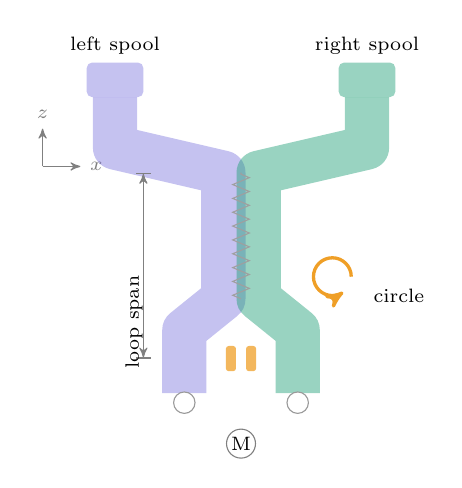
\begin{tikzpicture}[scale=0.80]
\axes \spools \ribbonszipped \mesh{2.20}{4.20} \mountclips \handsdefault \musician
\draw[->,amb,very thick] (5.75,2.55) arc (0:305:0.30);
\node[font=\scriptsize,anchor=west] at (5.95,2.25) {circle};
\draw[|<->|,gray] (2.45,1.25) -- (2.45,4.20);
\node[font=\scriptsize,anchor=east,rotate=90] at (2.30,2.72) {loop span};
\end{tikzpicture}
\caption{Loop. Mount to stopped front. Audition wide, cut narrow.}
\end{figure}

\subsection{Snip \normalfont(meta)}

\textbf{Both hands are involved.} One hand is nearest M, the other nearest the spools; what is
snipped is the section \emph{between the hands}.

\paragraph{The cut is virtual.} A \emph{copy} of the bracketed region is lifted into the tray. The
zipped band itself is undisturbed --- nothing is severed, nothing falls into the past, and no stub
is left clipped to the mount. Two consequences follow. M may take overlapping captures, the same
region twice, or work back over material she has already harvested; successive snips from one run
are therefore \emph{not} required to be adjacent. And the visual \MUST{} show the copy lifting
clear while the band remains whole, or M will expect a gap that is not there.

\begin{itemize}[leftmargin=*]
\item The near hand supplies $i_L$ and $i_R$; the separation of the hands in notches supplies $n$.
\item Roles are assigned by $z$-ordering at the moment of the gesture, \MUSTNOT{} by chirality.
      Either hand may be the near one.
\item Both boundaries \MUST{} lie inside the meshed span. Bracketing unmeshed lead would capture
      two unpaired ribbons rather than a tune.
\item The capture \MUST{} be previewed: while the pose is held, a marker tracks each hand along the
      band so M can slide to the right notch before closing.
\end{itemize}

M is free to capture a smaller section than the full extent from mount to front. The three
decisions are independent: the mount fixes where holding is taken over, the wave's stopping fixes
how much material exists, the capture fixes how much she keeps.

\paragraph{Silence is not captured.} A halt consumes no notches, so a capture spanning a halt
yields consecutive notes and the silence is absent from the tune. The silence is preserved in the
performance trace, which replays exactly. Carrying rests into captures is a deliberate deferral;
see \S\ref{sec:deferred}.

\paragraph{Naming.} A capture \MUST{} be auto-named at the moment it is taken, and \MUST{} be
renameable in the tray. M is in meta play with her hands free, so a prompt would interrupt nothing
--- but text entry on the headset is slow, and naming is a curatorial act rather than a performing
one. The \texttt{scissors} message therefore carries no name.

\begin{figure}[H]\centering
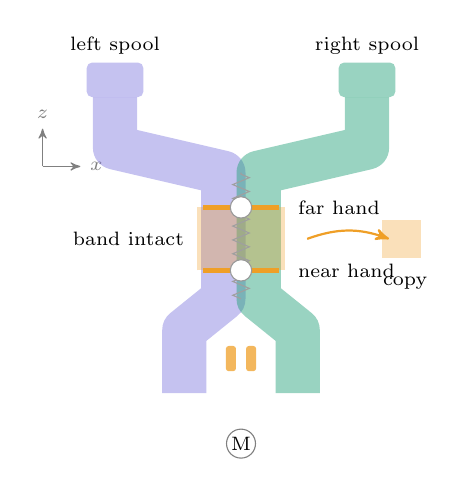
\begin{tikzpicture}[scale=0.80]
\axes \spools \ribbonszipped
\draw[amb,opacity=.32,line width=32pt] (4,2.65) -- (4,3.65);
\mesh{2.20}{4.20} \mountclips \musician
\draw[amb,line width=1.6pt] (3.40,2.65) -- (4.60,2.65);
\draw[amb,line width=1.6pt] (3.40,3.65) -- (4.60,3.65);
\handat{4.00}{2.65}\handat{4.00}{3.65}
\node[font=\scriptsize,anchor=west] at (4.75,2.65) {near hand};
\node[font=\scriptsize,anchor=west] at (4.75,3.65) {far hand};
\draw[amb,opacity=.32,line width=14pt] (6.55,2.85) -- (6.55,3.45);
\draw[->,amb,thick] (5.05,3.15) to[out=20,in=160] (6.35,3.15);
\node[font=\scriptsize,anchor=west] at (6.10,2.45) {copy};
\node[font=\scriptsize,anchor=east] at (3.25,3.15) {band intact};
\end{tikzpicture}
\caption{Snip. Two boundaries, both inside the mesh. A copy of what lies between the hands is
lifted to the tray; the band itself is untouched.}
\end{figure}

\subsection{Mutual exclusion}

\begin{itemize}[leftmargin=*]
\item The recogniser \MUST{} evaluate only the active mode's predicates.
\item Loop and pull \MUSTNOT{} be simultaneously satisfiable: a circling hand crosses the pull
      velocity threshold twice per revolution. Under the mode rule they never coexist, but the
      exclusion \MUST{} be explicit in case modes are ever relaxed.
\item Twist requires unzipped; zip and twist are never simultaneously satisfiable.
\item Every gesture \MUST{} be edge-triggered with a cooldown and \MUSTNOT{} re-fire while its pose
      is continuously held.
\end{itemize}

\subsection{Three kinds of detector}

The recogniser draws on three input sources and \MUST{} support three detector kinds. Only the
first exists today.

\begin{center}
\begin{tabular}{lll}
\toprule
\textbf{Kind} & \textbf{Source} & \textbf{Gestures} \\
\midrule
Per-frame pose  & hand anchors   & pull, twist, zip, unzip, mount, unmount, scissors \\
Trajectory      & hand anchors   & loop \\
Device pose     & head anchor    & halt \\
\bottomrule
\end{tabular}
\end{center}

The trajectory detector \MUST{} buffer index-fingertip positions over a window, fit a plane,
accumulate the unwrapped angle about the centroid, and fire when the sweep passes $2\pi$ with
radius variance and plane residual inside bounds. Direction of rotation comes free and gives
loop-set against loop-clear.

\subsection{Detection parameters}

Every threshold \MUST{} live in an external calibration profile, loaded at launch and reloadable
without a rebuild. Hardcoded constants \MUSTNOT{} remain in the recogniser.

\begin{center}
\begin{tabular}{lll}
\toprule
\textbf{Parameter} & \textbf{Governs} & \textbf{Provisional} \\
\midrule
\texttt{pull.velocity\_min}    & speed toward M            & 0.25 m/s \\
\texttt{pull.step\_divisor}    & speed to step count       & 0.15 \\
\texttt{pull.cooldown}         & minimum interval          & 0.08 s \\
\texttt{zip.distance}          & ribbons-together          & 0.10 m \\
\texttt{zip.closing\_window}   & tempo measurement window  & 0.30 s \\
\texttt{zip.frontier\_max}     & wave budget, in notches   & \emph{from reference device} \\
\texttt{unzip.distance}        & ribbons-apart             & 0.22 m \\
\texttt{twist.height\_delta}   & vertical offset           & 0.06 m \\
\texttt{twist.hold\_frames}    & frames before firing      & 8 \\
\texttt{halt.roll\_fire}       & head roll, firing angle   & $15^\circ$ \\
\texttt{halt.roll\_rearm}      & head roll, re-arm angle   & $6^\circ$ \\
\texttt{halt.hold}             & hold before firing        & 0.25 s \\
\texttt{scissors.spread}       & index/middle angle        & 0.40 rad \\
\texttt{scissors.extended}     & extension floor           & \emph{to be derived} \\
\texttt{scissors.curled}       & curl ceiling              & \emph{to be derived} \\
\texttt{loop.min\_radius}      & circle size floor         & \emph{to be derived} \\
\texttt{loop.radius\_variance} & circularity tolerance     & \emph{to be derived} \\
\texttt{loop.plane\_residual}  & planarity tolerance       & \emph{to be derived} \\
\bottomrule
\end{tabular}
\end{center}

\subsection{Finger curl must be scale-invariant}

The implemented curl metric is $\lVert\text{tip}-\text{metacarpal}\rVert/0.08$ clamped to unity,
with ``curled'' asserted below $0.30$. A fully curled adult ring finger measures roughly
$0.06$--$0.08$\,m tip-to-metacarpal, giving $0.75$--$1.0$. The threshold is unreachable and
scissors never fires. The metric is also not scale-invariant: the fixed divisor makes detection
depend on hand size.

Curl \MUST{} instead be the interior angle at the proximal interphalangeal joint, or tip-to-wrist
distance normalised by that finger's own summed segment lengths. Thresholds \MUST{} be derived from
recorded traces (\S\ref{sec:instrumentation}), not chosen by inspection.


\section{Snip semantics and the tune term}
\label{sec:snip}

\subsection{The defect being corrected}

The engine currently derives a snip from the \emph{left} cursor alone: it computes
$\textit{from}=p_L-w$ and $\textit{to}=p_L$ for ribbon width $w$, then advances both fresh spigots
to \textit{from}. Since $p_L$ and $p_R$ are independent by design, the stored snippet is
$(d(c_L,b_L,k), d(c_R,b_R,k))_{k}$ over a single index, while what M heard was
$(d(c_L,b_L,i), d(c_R,b_R,j))$ with $i$ and $j$ independent.

\begin{quote}\itshape
A snipped tune is, in general, not the tune M heard.
\end{quote}

A third representation compounds it: the tray receives the digits actually displayed, while the
snippet map receives the re-derived pairs. ``The snipped tune'' denotes three different things
depending on where one looks.

\subsection{Resolution}

\[
\mathsf{Snip}(k,\; i_L,\; i_R,\; n)
\quad\text{denoting}\quad
\big(d(c_L,b_L,i_L+t),\ d(c_R,b_R,i_R+t)\big)_{t\in[0,n)} .
\]

The mesh guarantees equal counts on both sides, so a common length $n$ is exact rather than
assumed. The near hand supplies $i_L$ and $i_R$; the hand separation supplies $n$. Tray, snippet map
and realised audio \MUST{} all derive from this one term.

\subsection{Consequences}

\paragraph{The Theory of skeins.} \texttt{Skein.module} currently declares
\begin{lstlisting}
Snip . k:Skein, i:Nat, j:Nat |- "snip" "(" k "," i "," j ")" : Tune;
\end{lstlisting}
inheriting the single-interval assumption. It becomes
\begin{lstlisting}
Snip . k:Skein, iL:Nat, iR:Nat, n:Nat
     |- "snip" "(" k "," iL "," iR "," n ")" : Tune;
\end{lstlisting}
with the empty-snip equation restated as
$(\mathsf{Snip}\ k\ i_L\ i_R\ \mathsf{NZero}) == (\mathsf{Rest})$. A cut placed with the hands
together gives $n=0$ and normalises to $\mathsf{Rest}$ by that equation.

\paragraph{Twist commutes with snipping, for free.}
\begin{proposition}
Normalising $\mathsf{Twist}(\mathsf{Wv}\ l\ r)$ to $\mathsf{Wv}\ r\ l$ also reinterprets $i_L$ as
indexing $r$, which is what the engine does---twist swaps whole spigots, configuration and cursor
together. No additional equation is required.
\end{proposition}

\paragraph{A run yields a family of tunes.} Because the cut is virtual the band is never
disturbed, so M may capture any windows she likes over one mesh: $\mathsf{Snip}(k,i_L+a,i_R+a,m)$
for any offset $a$ and length $m$ inside the meshed span. They need not be adjacent, need not be
disjoint, and may repeat. The relation between a performance and the tunes taken from it is
readable off the syntax rather than stored in a link table---the same argument that made tunes
terms in the first place---and overlap is visible in the syntax as shared intervals.

\subsection{Interpretation lives in the envelope}
\label{sec:envelope}

Since the pitch and duration maps are changeable during a session (\S\ref{sec:maps}), the term
alone is underdetermined: the same $\mathsf{Snip}(k,i_L,i_R,n)$ sounds different under a different
scale. The split is clean and \MUST{} be observed:

\begin{center}
\begin{tabular}{ll}
\toprule
\textbf{The term} & \textbf{The envelope} \\
\midrule
which digits, paired how & pitch map, duration map, tempo, instrument \\
$\mathsf{Snip}(k,i_L,i_R,n)$ & copied in at capture time \\
\bottomrule
\end{tabular}
\end{center}

The term is the material; the envelope is the interpretation. Breeding therefore operates on
material and is map-agnostic, which is what is wanted when crossing two tunes made in different
scales.

\section{Performance recording}

\begin{definition}[Performance trace]
An ordered sequence of timestamped records: an opening declaration of both stream configurations,
the maps, tempo and instrument; then every gesture event with its parameters; then a closing
timestamp.
\end{definition}

The engine \MUST{} record a trace for every session without being asked. The streams are
deterministic and the state machine is total, so the trace \MUST{} replay the session exactly; no
audio is stored. Snips \MUST{} appear in the trace, so a performance resolves to the tunes harvested
from it and each tune resolves back to its performance. Timestamps \MUST{} be monotonic at
millisecond resolution or better, and records \SHOULD{} carry the raw hand-tracking metrics that
produced each gesture, for \S\ref{sec:instrumentation}.

\section{Wire protocol, version 3}
\label{sec:protocol}

Messages \MUST{} be newline-delimited JSON, one object per line, each carrying \texttt{type} and
\texttt{"v": 3}. Both sides \MUST{} serialise via \texttt{Codable} and \texttt{serde}; neither side
\MAY{} construct JSON by string interpolation. The current client escapes only the double quote, so
a name containing a backslash produces malformed JSON that the engine silently discards.

\subsection{Client to engine}

\begin{center}
\begin{tabular}{l>{\raggedright\arraybackslash}p{4.6cm}l}
\toprule
\textbf{Type} & \textbf{Fields} & \textbf{Note} \\
\midrule
\texttt{pull\_left}, \texttt{pull\_right} & \texttt{steps}, \texttt{velocity} & \\
\texttt{twist}     & --- & rejected unless unzipped \\
\texttt{zip}       & \texttt{closing\_speed} & sets the mesh tempo \\
\texttt{unzip}     & --- & \\
\texttt{halt}      & \texttt{on} & from roll direction; not a toggle \\
\texttt{mount}     & --- & stops the wave; enters meta \\
\texttt{unmount}   & --- & returns to play; mesh survives \\
\texttt{loop}      & \texttt{on} & from rotation direction \\
\texttt{scissors}  & \texttt{near}, \texttt{far} & two notch offsets; no name \\
\texttt{rename}    & \texttt{id}, \texttt{name} & tray operation \\
\texttt{configure} & \texttt{left}, \texttt{right}, \texttt{pitch\_map},
                     \texttt{duration\_map}, \texttt{tempo}, \texttt{instrument} & \\
\texttt{quit}      & --- & \\
\bottomrule
\end{tabular}
\end{center}

Three substantive changes. \texttt{scissors} carries two notch offsets, where the gesture
currently fires a locationless event and the engine derives the window from the ribbon width---the
assumption revision 3 removed. \texttt{zip} carries the closing speed, which is the tempo.
\texttt{halt} and \texttt{loop} carry a direction-derived boolean rather than toggling, so a
missed or doubled fire cannot invert the state.

\subsection{Engine to client}

\begin{center}
\begin{tabular}{l>{\raggedright\arraybackslash}p{9.2cm}}
\toprule
\textbf{Type} & \textbf{Fields} \\
\midrule
\texttt{digits}    & \texttt{left}, \texttt{right}, \texttt{left\_pos}, \texttt{right\_pos} \\
\texttt{note}      & \texttt{pitch}, \texttt{duration}, \texttt{velocity},
                     \texttt{left\_pos}, \texttt{right\_pos}, \texttt{notch\_index} \\
\texttt{zip\_state}& \texttt{zipped}, \texttt{front}, \texttt{running}, \texttt{tempo},
                     \texttt{budget\_left}, \texttt{stopped\_by} \\
\texttt{snip\_ack} & \texttt{id}, \texttt{name}, \texttt{count}, \texttt{i\_left}, \texttt{i\_right} \\
\texttt{state}     & \texttt{mode}, \texttt{looping}, \texttt{left\_label},
                     \texttt{right\_label}, \texttt{pitch\_map}, \texttt{duration\_map},
                     \texttt{instrument} \\
\texttt{status}    & \texttt{text} \\
\texttt{error}     & \texttt{code}, \texttt{text} \\
\bottomrule
\end{tabular}
\end{center}

\texttt{stopped\_by} \MUST{} distinguish \texttt{halt}, \texttt{mount} and
\texttt{exhausted}. The wave can now end without a gesture, and a run that stops mid-phrase with
no explanation reads as a crash; the client \MUST{} also give a visible approach signal as
\texttt{budget\_left} runs down. Playback state \MUST{} be a field, never inferred from prose. The client currently clears its
playing flag on \texttt{statusText.contains("stopped")}. Nothing in the client \MAY{} parse
\texttt{status}, which is advisory and human-readable only.

\subsection{Rate discipline}

The engine currently emits \texttt{status} on every frame of its 60\,Hz loop, beneath a comment
reading ``Push status if changed'' describing a check the code does not perform. Each message
invalidates the entire client panel.

\begin{itemize}[leftmargin=*]
\item \texttt{status}, \texttt{state} and \texttt{zip\_state} \MUST{} be emitted only on change.
\item \texttt{digits} \MUST{} be emitted only when a cursor moves, coalesced to at most 30\,Hz.
\item \texttt{note} \MUST{} be emitted per note and \MUSTNOT{} be coalesced.
\item Aggregate steady-state traffic \SHOULD{} stay below 200 messages per second.
\end{itemize}

\section{Visual model}

\paragraph{Axis correction.} \texttt{RibbonView.swift} places both ribbons at a shared
\texttt{RIBBON\_X} and separates them by \texttt{LEFT\_Y}/\texttt{RIGHT\_Y}---stacked vertically at
the same left-right position. Under \S\ref{sec:surface} they separate on \textbf{$x$}, left spool
to the left hand. This \MUST{} be corrected before any geometry is tuned.

\paragraph{Patches.} Pooled and reused. Text meshes and materials \MUST{} be cached per digit value
and per depth bucket and \MUSTNOT{} be regenerated per frame; \texttt{PatchEntity.configure}
currently calls \texttt{MeshResource.generateText} and builds a fresh physically-based material for
every patch on every update, which is the dominant cost in the render path.

\paragraph{The three sections} \MUST{} be visually distinct: future occluded on the spool, present
taut and legible, past hanging below the hands and dimmed.

\paragraph{The mesh} \MUST{} be rendered at the notch scale. The zip front \MUST{} be a distinct,
clearly visible entity, since it is the playhead M watches. It no longer needs to be
\emph{targetable}: halt is a head gesture, so nothing aims at the front, and any minimum apparent
size is an aesthetic choice rather than a functional requirement.

\paragraph{Far-field compression.} As the wave runs, the spools \MUST{} compress toward point
sources well before the frontier budget is exhausted, so that the cost of a long play is visible
in $z$-axis real estate. The compression \MUST{} be continuous; a discontinuity will read as a
glitch.

\paragraph{The virtual cut} \MUST{} be rendered as a copy lifting clear of an intact band. Showing
a gap, a severed end or a falling stub would misrepresent the mechanism and lead M to expect
material to be consumed.

\paragraph{Hand ghosts} \MUST{} mirror the tracked joints. The recogniser receives every hand anchor
and discards it; the ghost entity is added to the scene and never updated.

\paragraph{The tray} \MUST{} display the digits actually snipped, not the live ribbon contents.

\section{Audio model}

Audio \MUST{} be synthesised on the headset. In the current architecture the engine drives CoreMIDI
on the Mac, so M pulls a ribbon in front of her face and hears the result from a laptop across the
room, after a network hop and a MIDI buffer. That makes the latency figure---the most important
measurement of the September sessions---unrepresentative of any shipping configuration.

\begin{itemize}[leftmargin=*]
\item The client \MUST{} render \texttt{note} messages through an on-device sampler.
\item Audio \SHOULD{} be spatialised so each ribbon sounds from its own position. The two streams
      are distinct objects in front of M and should be audibly distinct.
\item Mac-side MIDI \MAY{} be retained for recording to a workstation and \MUSTNOT{} be the default.
\end{itemize}

\section{Non-functional requirements}

\begin{center}
\begin{tabular}{lll}
\toprule
\textbf{Property} & \textbf{Target} & \textbf{Maximum} \\
\midrule
Notch engagement to audible note & 30 ms & 50 ms \\
Head roll to front freezing & one frame & two frames \\
Gesture to visual response & one frame & two frames \\
Rendered frame rate & 90 fps sustained & --- \\
Digit emission, memoised range & --- & 1 ms per 1000 digits \\
Engine to client message rate & $<$100 s\textsuperscript{-1} & 200 s\textsuperscript{-1} \\
Session length without degradation & 45 min & --- \\
\bottomrule
\end{tabular}
\end{center}

Failure modes \MUST{} be visible and recoverable. Channel loss \MUST{} surface in the panel and
retry with backoff, preserving engine state. Denial of hand-tracking authorization \MUST{} produce
an explanatory message and fall back to panel controls, not a console line. The tray \MUSTNOT{}
silently discard entries; it currently caps at twenty and drops the oldest.

\section{Instrumentation}
\label{sec:instrumentation}

The thresholds are guesses, one is provably unreachable, and there is no data to tune against.

\begin{itemize}[leftmargin=*]
\item A debug overlay \MUST{} display live metrics per hand: separation, palm velocity, height
      differential, per-finger extension and curl, accumulated rotation angle, and which predicates
      are satisfied.
\item Raw joint transforms \MUST{} be recordable at tracking rate with a manual label marker.
\item Thresholds \MUST{} be tunable offline and reloadable without a rebuild.
\end{itemize}

The first half-day of headset time \SHOULD{} capture a labelled corpus rather than play. Those
traces are the same artifact as a performance trace, so the work is a first delivery of the product
rather than a detour from it.

\section{Publishing and consent}

Everything the instrument produces --- tunes, performance traces, gesture corpora --- is M's, and
her back-end data is guarded by her private key. Recording every session by default is therefore
safe: nothing becomes visible to anyone else without an explicit publishing action taken by M.

\begin{itemize}[leftmargin=*]
\item The engine \MUST{} record every session's performance trace without asking.
\item No artifact \MAY{} leave the device, or become visible to any other party, except through an
      explicit publish action.
\item Publishing \MUST{} be a distinct, deliberate act, never a side effect of capture, naming, or
      any gesture in \S\ref{sec:gestures}.
\end{itemize}

\section{Deferred}
\label{sec:deferred}

Recorded here so the reasoning is not lost.

\paragraph{Rests in captures.} A halt places a silence that is preserved in the performance trace
but absent from any tune captured across it. Carrying the silence would be expressible with
machinery the theory already has --- since a mesh has one tempo, a wall-clock halt quantises to a
definite number of rests, and the capture becomes
$\mathsf{Seq}[\mathsf{Snip}(k,i_L,i_R,a),\ \mathsf{Rest}^{\,m},\ \mathsf{Snip}(k,i_L{+}a,i_R{+}a,b)]$
with no new constructors. It is deferred because it makes a capture no longer always a single leaf,
and tunes with differing internal structure are harder to cross than flat runs. Revisit after the
breeding engine is exercised.

\paragraph{Gestural map control.} Changing pitch and duration maps by gesture rather than by text.
Deferred to keep the vocabulary at ten.

\section{Conformance checklist}

\begin{enumerate}[leftmargin=*,itemsep=0.15em]
\item Clean install on device; entitlements and provisioning verified.
\item Hand-tracking authorization requested, granted, denial handled visibly.
\item Device-pose authorization confirmed and granted.
\item Engine discovered automatically; connection indicated within five seconds.
\item All ten gestures fire, each confirmed in the debug overlay, before any music is attempted.
\item Hand ghosts visible and tracking.
\item Zip propagates unaided; each notch pair sounds from the headset; spools compress as it runs.
\item Closing the hands faster yields an audibly faster run.
\item Head roll one way freezes the front, the other resumes, and repeats in the same direction are
      no-ops.
\item Tempo is unchanged across a halt and resume.
\item The wave stops of its own accord at the frontier, with an approach signal beforehand and
      \texttt{stopped\_by} reporting \texttt{exhausted}.
\item Mount stops the wave and enters meta; unmount returns to play with the mesh intact.
\item Pull, twist, zip and unzip do not fire in meta; loop and scissors do not fire in play.
\item Loop set and cleared by rotation direction; loop span runs mount to front.
\item Snip with two hands yields a tune of exactly the bracketed notch count, auto-named.
\item The band is visibly intact after a snip, and a second overlapping snip succeeds.
\item A captured tune, re-realised from $(k,i_L,i_R,n)$ under its envelope, is identical to what was
      heard.
\item A capture spanning a halt contains no silence; the performance trace replays the silence.
\item 90 fps sustained with sixty patches per ribbon.
\item Tray and performance trace survive an application restart.
\item Gesture traces written to disk.
\end{enumerate}

Items 17 and 18 are the acceptance tests for \S\ref{sec:snip}; neither can pass on the current
build.

\section{Triage against the demo deadline}
\label{sec:demo}

Not all of this is needed to demonstrate the instrument. Ranked by what a demo actually requires:

\paragraph{Blocking --- without these there is no demo.} Transport off the Unix socket
(\S2); on-device audio (\S13); the scale-invariant curl metric, without which scissors cannot fire
at all; the four unwired visual features; and the axis correction, since the ribbons are currently
stacked on $y$.

\paragraph{Core to the idea.} Zip with propagation and tempo from closing; halt by head roll;
mount, unmount and the mode split; the two-handed virtual snip.

\paragraph{Deferrable if time runs short.} Loop, which needs the trajectory detector --- the
demo survives without it, though auditioning before capture is a large part of what makes the
instrument feel like an instrument. Far-field compression, which is expressive rather than
functional. Textual map control, if a single sensible default scale is chosen. The frontier bound,
if the demo runs are short.

\paragraph{Not deferrable despite looking like it.} The gesture-trace recorder. Every threshold in
\S6.12 is a guess, and without recorded traces the tuning after the first session will be guesswork
too.

\section{Decisions sought}
\label{sec:decisions}

The ten decisions raised by revision 3 are settled and incorporated. What remains:

\begin{enumerate}[leftmargin=*,itemsep=0.4em]
\item \textbf{The frontier figure.} \texttt{zip.frontier\_max} is specified as ``a generous looper
      phrase''. Set the number from a reference device.
\item \textbf{Roll thresholds.} $15^\circ$ firing and $6^\circ$ re-arm are provisional and should be
      confirmed against recorded traces --- players lean into phrases, and the false-fire rate is
      unknown.
\item \textbf{Auto-naming scheme.} Take number, or a name derived from the address itself. The
      latter is more informative and less legible.
\item \textbf{Default maps.} Which pitch and duration map, over which root, when a session opens.
\item \textbf{Configuration ordering.} S1 tethered for the demo with S2 to follow, or straight to
      S2. About three days against about a week, with the demo deadline the deciding factor.
\end{enumerate}

\end{document}
